\documentclass[12pt,a4paper]{article}
\usepackage[warn]{mathtext}
\usepackage[utf8]{inputenc}
\usepackage[english,russian]{babel}
\usepackage{amsmath}
\usepackage{amssymb}
\usepackage{latexsym}
\usepackage{svg}
\usepackage{indentfirst}
\usepackage{pgfplots}
\pgfplotsset{compat=1.9}

\usepackage{listings}

\usepackage{color}

\definecolor{dkgreen}{rgb}{0,0.6,0}
\definecolor{gray}{rgb}{0.5,0.5,0.5}
\definecolor{mauve}{rgb}{0.58,0,0.82}

\lstset{ %
	language=C++,                % Язык программирования 
	numbers=left,                   % С какой стороны нумеровать
	stepnumber=1,                   % Шаг между линиями. Если 1, то будет пронумерована каждая строка
	frame=single,	
}
\usepackage[left=2cm,right=2cm,
top=2cm,bottom=2cm,bindingoffset=0cm]{geometry}

\usepackage{sverb}
\usepackage{graphicx}
\usepackage{pdfpages}
\usepackage[absolute,overlay]{textpos}
\usepackage{setspace}
\onehalfspacing
\numberwithin{equation}{section}

\begin{document}
	\begin{titlepage}
		\begin{textblock*}{13cm}(0cm,0cm)
			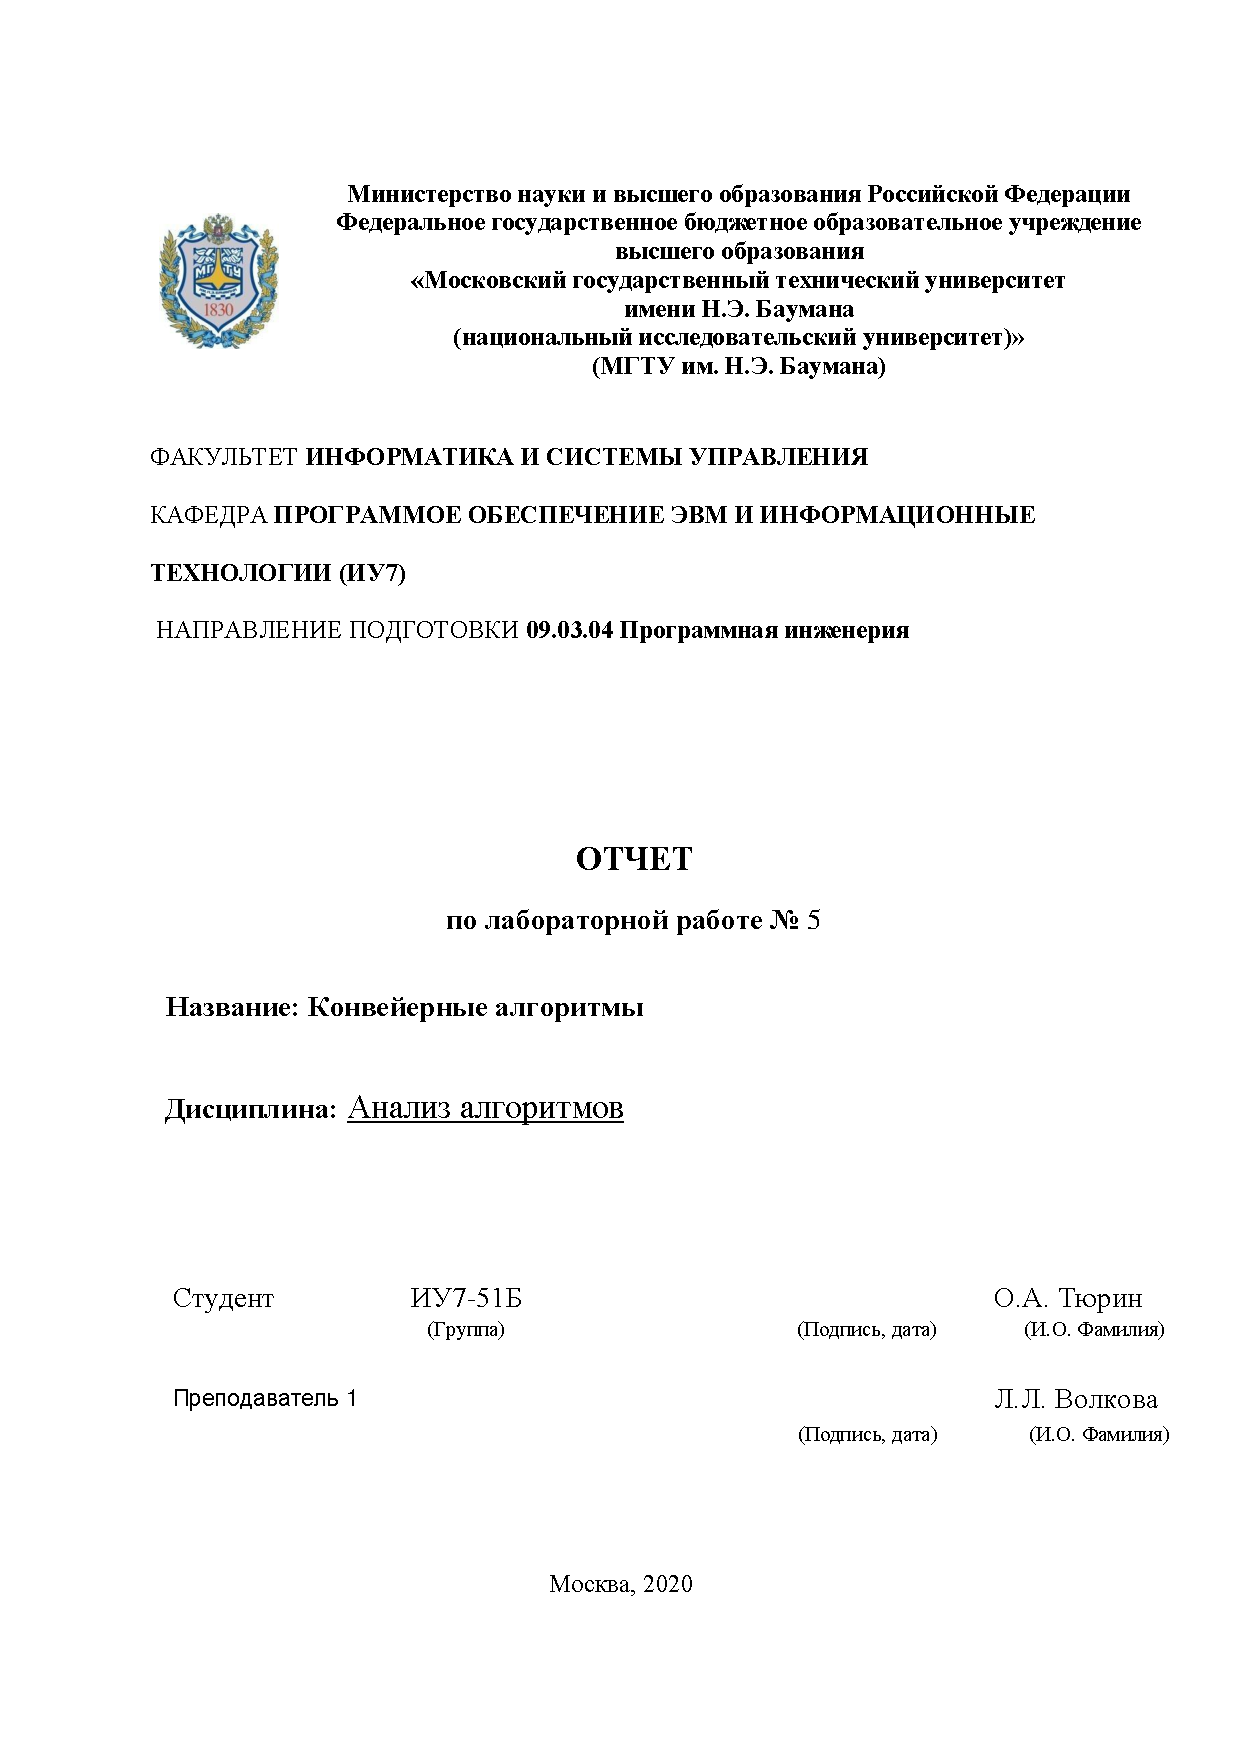
\includegraphics{reportTitle}
		\end{textblock*}
	\end{titlepage}
\hspace{0pt}
\clearpage
%	\begin{titlepage}
%		\centering
%		\Huge Лабораторная работа №1 по курсу \\\textbf{"Анализ алгоритмов"}\\
%		Тема: Расстояния Левенштейна и Дамерау-Левенштейна\\
%		\vspace{\baselineskip}
%		\Large Работу выполнил: Колосов Д.В ИУ7-52Б\\
%		Преподаватели: Волкова Л.Л, Строганов Ю.В.
%		\vfill
%		Москва, 2020 г.		
%	\end{titlepage}
\tableofcontents
\clearpage

\addcontentsline{toc}{section}{Введение}
%//////////////////////////////////////////////////////////////////
\section*{\Huge Введение}
Выполнение каждой команды складывается из ряда последовательных шагов суть
которых не меняется от команды к команде. С целью увеличения быстродействия про-
цессора и максимального использования всех его возможностей в современных микро-
процессорах используется конвейерный принцип обработки информации. Этот принцип
подразумевает, что в каждый момент времени процессор работает над различными стади-
ями выполнения нескольких команд, причем на выполнение каждой стадии выделяются
отдельные аппаратные ресурсы. По очередному тактовому импульсу каждая команда в
конвейере продвигается на следующую стадию обработки, выполненная команда покидает
конвейер, а новая поступает в него.\\\\
Целью лабораторной работы является создание системы конвейерной обработки.\\
Задачами данной лабораторной работы являются:\\
\begin{itemize}
	\item спроектировать ПО, реализующего конвейерную обработку;
	\item описать реализацию ПО;
	\item провести тестирование ПО.
\end{itemize}

В ходе данной лабораторной работы будут изучены возможности конвейерных вычислений и использование подобного подхода на практике.
\clearpage

\section{Аналитическая часть}
В данном разделе будут рассмотрены общие сведения о конвейерной обработке и произ-
ведена оценка производительности конвейера.

\subsection{Конвейерная обработка}
\qquad Конвейер — способ организации вычислений, используемый в современных процес-
сорах и контроллерах с целью повышения их производительности (увеличения числа ин-
струкций, выполняемых в единицу времени).
Один из самых простых и наиболее распространенных способов повышения быстро-
действия процессоров — конвейеризация процесса вычислений.
Конвейеризация – это техника, в результате которой задача или команда разбивается
на некоторое число подзадач, которые выполняются последовательно. Каждая подкоман-
да выполняется на своем логическом устройстве. Все логические устройства (ступени)
соединяются последовательно таким образом, что выход i-ой ступени связан с входом
(i+1)-ой ступени, все ступени работают одновременно. Множество ступеней называется
конвейером. Выигрыш во времени достигается при выполнении нескольких задач за счет
параллельной работы ступеней, вовлекая на каждом такте новую задачу или команду.

\subsection{Оценка производительности конвейера}
\qquad Пусть задана операция, выполнение которой разбито на n последовательных этапов. При последовательном их выполнении операция выполняется за время

\begin{equation}\label{form:way}
 \tau _{e}={\sum\limits_{i=1}^n \tau _{i}}
 \end{equation}
 \begin{align*}
    \text{где} \\
    n &- \text{количество последовательных этапов;} \\
   \tau _{i} &- \text{время выполнения i-го этапа;}
\end{align*}

Быстродействие одного процессора, выполняющего только эту операцию, составит

\begin{equation}\label{form:way}
 S_{e}={\frac{1}{\tau _{e}}}={\frac{1}{\sum\limits_{i=1}^n \tau _{i}}}
 \end{equation}
 \begin{align*}
    \text{где} \\
    \tau _{e} &- \text{время выполнения одной операции;} \\
    n &- \text{количество последовательных этапов;} \\
   \tau _{i} &- \text{время выполнения i-го этапа;}
\end{align*}

Выберем время такта — величину $t _{T} = max{\sum\limits_{i=1}^n(\tau_{i})}$ и потребуем при разбиении на этапы, чтобы для любого i = 1, ... , n выполнялось условие $(\tau_{i} + \tau_{i+1}) mod n = \tau_{T}$. То есть чтобы никакие два последовательных этапа (включая конец и новое начало операции) не могли быть выполнены за время одного такта.

Максимальное быстродействие процессора при полной загрузке конвейера составляет

\begin{equation}\label{form:way}
 S_{max}={\frac{1}{\tau _{T}}}
 \end{equation}
 \begin{align*}
    \text{где} \\
    \tau _{T} &- \text{выбранное нами время такта;}
\end{align*}

Число n — количество уровней конвейера, или глубина перекрытия, так как каждый такт на конвейере параллельно выполняются n операций. Чем больше число уровней (станций), тем больший выигрыш в быстродействии может быть получен.

Известна оценка
\begin{equation}\label{form:way}
{\frac{n}{n/2} \leq {\frac{S_{max}}{S_{e}}} \leq n}
 \end{equation}
 \begin{align*}
    \text{где} \\
    S_{max} &- \text{максимальное быстродействие процессора  при полной загрузке конвейера;} \\
    S_{e} &- \text{стандартное быстродействие процессора;} \\
   n &- \text{количество этапов.}
\end{align*}

то есть выигрыш в быстродействии получается от n/2  до n раз [2].


Реальный выигрыш в быстродействии оказывается всегда меньше, чем указанный выше, поскольку:

\begin{enumerate}
\item[1)] некоторые операции, например, над целыми, могут выполняться за меньшее количество этапов, чем другие арифметические операции. Тогда отдельные станции конвейера будут простаивать;
\item[2)] при выполнении некоторых операций на определённых этапах могут требоваться результаты более поздних, ещё не выполненных этапов предыдущих операций. Приходится приостанавливать конвейер;
\item[3)] поток команд(первая ступень) порождает недостаточное количество операций для полной загрузки конвейера.
\end{enumerate}

\subsection{Параллельное программирование}
При использовании многопроцессорных вычислительных систем с общей памятью обычно предполагается, что имеющиеся в составе системы процессоры обладают равной производительностью, являются равноправными при доступе к общей памяти, и время доступа к памяти является одинаковым (при одновременном доступе нескольких процессоров к одному и тому же элементу памяти очередность и синхронизация доступа обеспечивается на аппаратном уровне). Многопроцессорные системы подобного типа обычно именуются симметричными мультипроцессорами (symmetric multiprocessors, SMP) \cite{litlink3}.\\

Обычный подход при организации вычислений для многопроцессорных вычислительных систем с общей памятью – создание новых параллельных методов на основе обычных
последовательных программ, в которых или автоматически компилятором, или непосредственно программистом выделяются участки независимых друг от друга вычислений. Возможности автоматического анализа программ для порождения параллельных вычислений достаточно ограничены, и второй подход является преобладающим.\\

Широко используемый подход состоит и в применении тех или иных библиотек, обеспечивающих определенный программный интерфейс (application programming interface,
API) для разработки параллельных программ. В рамках такого подхода наиболее известны Windows Thread API \cite{litlink1}. Однако первый способ применим только для ОС семейства
Microsoft Windows, а второй вариант API является достаточно трудоемким для использования и имеет низкоуровневый характер

\subsection {Организация взаимодействия параллельных потоков}
Как уже было сказано, потоки, в отличии от процессов, не имеют собственного адресного пространства. Как результат, взаимодействи потоков можно реализовать через использование общих данных. В случае, когда общие данные необходимо только читать - проблем возникнуть не может. В случае, если необходимо общие данные изменять - необходимо пользоваться \textbf{средствами синхронизации}: mutex, семафор.

\subsection{Конвейерный алгоритм без многопоточности}
Есть последовательность строк, длиной n.\\
Чтобы подсчитать количество вхождений каждого символа в каждой строке, необходимо создать n дополнительных массивов, каждый из которых имеет размерность m (m - мощность некого алфавита, на основе которого строятся строки).
Далее необходимо проитерировать каждую из строк и инкрементировать соответствующую ячейку массива.\\
Пример:
\begin{center}
	strings = \{"qwer"{}, "asdf"{}, "zxcv"{}\}
\end{center}
Все строки составляются из английских строчных букв. Следжовательно мощность алфавита - 26.\\
Создаем дополнительные массивы размерностью 26:
\begin{center}
	arr1 = arr2 = arr3 = [26]\\
\end{center}
Возьмем 2 конвейера. Тогда каждый из конвейеров должен обработать свою часть.\\
Так как конвейеров 2, то каждый из конвейеров должен обработать по половине каждой строки.\\

\textbf{Конвейер 1:} \qquad\qquad\qquad\qquad\qquad\qquad\qquad\qquad\qquad\qquad \textbf{Конвейер 2:}  \\\\
\begin{center}
	"qwer"\\
\end{center}
arr1['q'] = arr1['q'] + 1 \qquad\qquad\qquad\qquad\qquad\qquad\qquad\qquad arr1['e'] = arr1['c'] + 1\\
arr1['w'] = arr1['w'] + 1 \qquad\qquad\qquad\qquad\qquad\qquad\qquad\qquad
arr1['r'] = arr1['d'] + 1\\\\

\begin{center}
	"asdf"\\
\end{center}
arr2['a'] = arr2['a'] + 1 \qquad\qquad\qquad\qquad\qquad\qquad\qquad\qquad
arr2['d'] = arr2['f'] + 1\\
arr2['s'] = arr2['s'] + 1 \qquad\qquad\qquad\qquad\qquad\qquad\qquad\qquad
arr2['f'] = arr2['d'] + 1\\\\

\begin{center}
	"zxcv"\\
\end{center}
arr3['z'] = arr3['z'] + 1 \qquad\qquad\qquad\qquad\qquad\qquad\qquad\qquad
arr3['c'] = arr3['j'] + 1 \\
arr3['x'] = arr3['x'] + 1 \qquad\qquad\qquad\qquad\qquad\qquad\qquad\qquad
arr3['v'] = arr3['i'] + 1\\

Таким образом в каждом из соответствуюших массивов хранится колчиство вхождений каждого из символов алфавита в соответствующей строке.

\subsection{Конвейерный алгоритм с использованием многопоточности}
В целом алгоритм, в основе которого лежит использование множества потоков является схожим с последовательным алгоритмом с той лишь разницей, что потоки делят между собой адресное пространство. Таким образом, в отличие от последовательного алгоритма можно не дожидаться пока каждый из конвейеров обработает \textbf{все} стркои, а передавать \textbf{уже обработанные} строки на обработку следующему конвейеру.

\subsection{Вывод}
В данном разделе были рассмотрены основы конвейерной обработки и произведена оценка
производительности конвейера.
\clearpage

\section{Конструкторская часть}
\subsection{Описание алгоритмов}
\qquad В данном разделе будут описан каждый исследуемый алгоритм.\\

\textbf{Требования к вводу}: на вход подаётся количество строк и сами строки.\\
\textbf{Требования к программе}: Подсчёт количество вхождений каждого символа в каждой строке.


\clearpage
\subsection{Разработка алгоритмов} % Сюда схемы алгоритмов
В данном разделе представлены схемы реализуемых алгоритмов.\\
На рисунке 2.1 представлена схема последовательного конвейерного алгоритма подсчёта.\\
\begin{center}	
	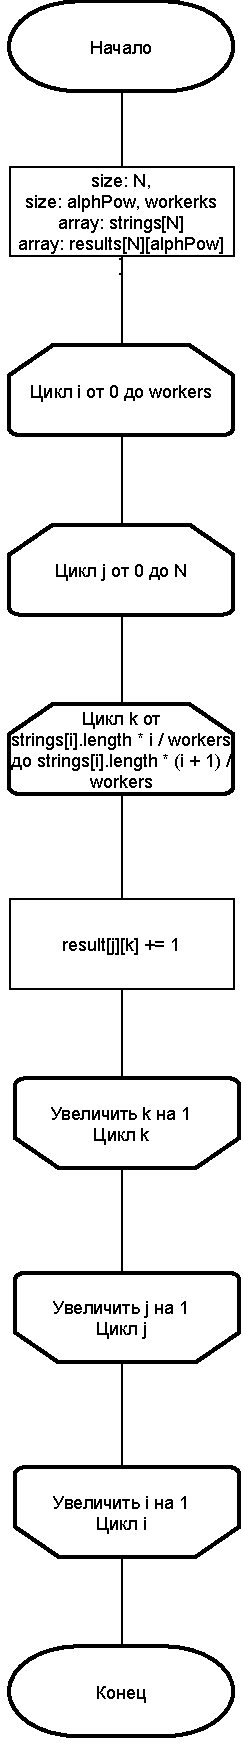
\includegraphics[width=.18\linewidth]{src/schemas/consistent}\\
	Рис. 2.1: Cхема последовательного конвейерного алгоритма подсчёта
\end{center}
\clearpage
На рисунке 2.2.1 представлена схема главного потока параллельного конвейерного алгоритма.\\
\begin{center}	
	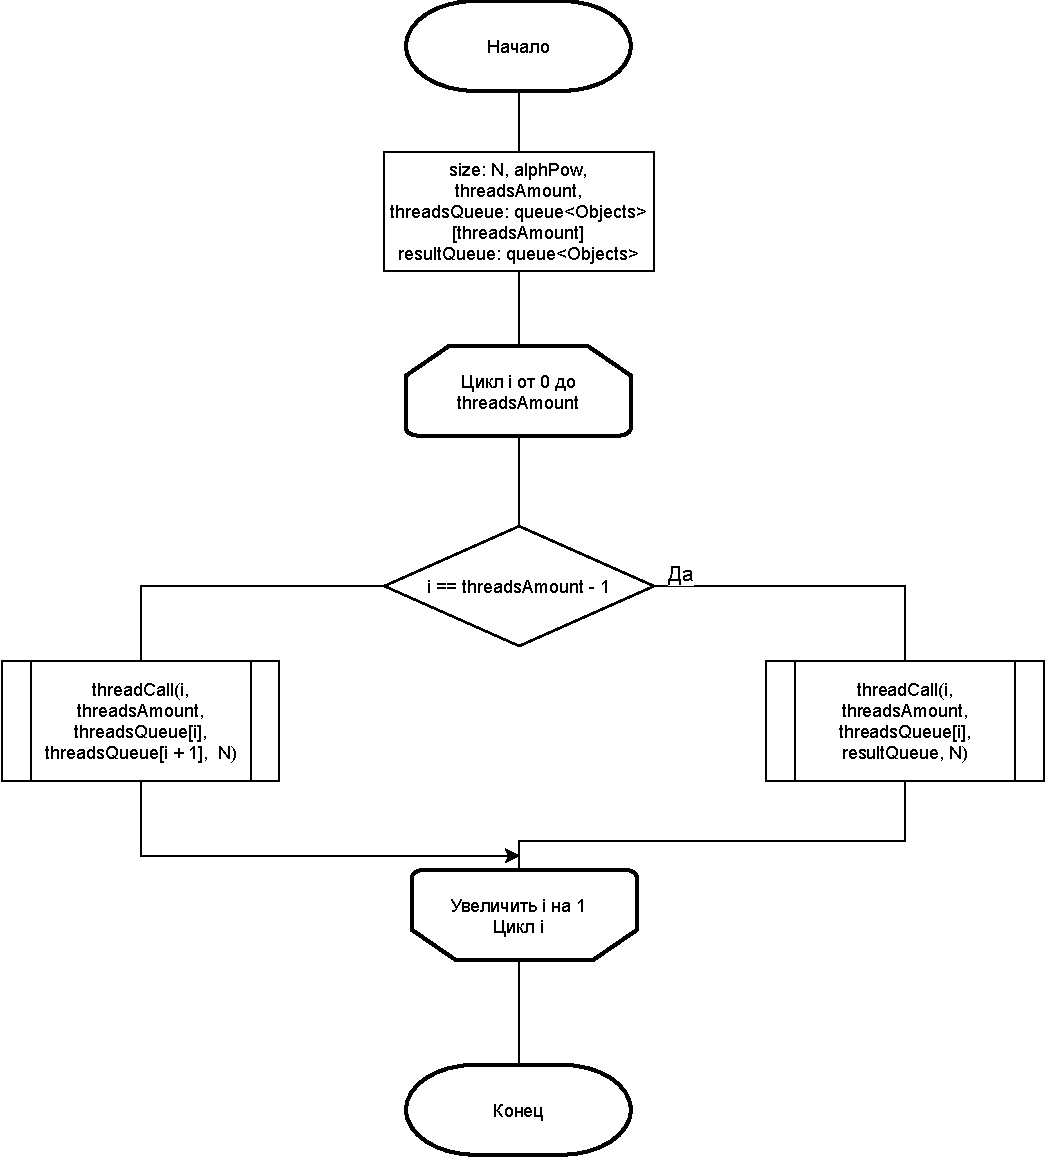
\includegraphics[width=1\linewidth]{src/schemas/parallel_main}\\
	Рис. 2.2.1: Cхема главного потока параллельного конвейерного алгоритма
\end{center}
\clearpage
На рисунке 2.2.2 представлена схема дочернего потока параллельного конвейерного алгоритма.\\
\begin{center}	
	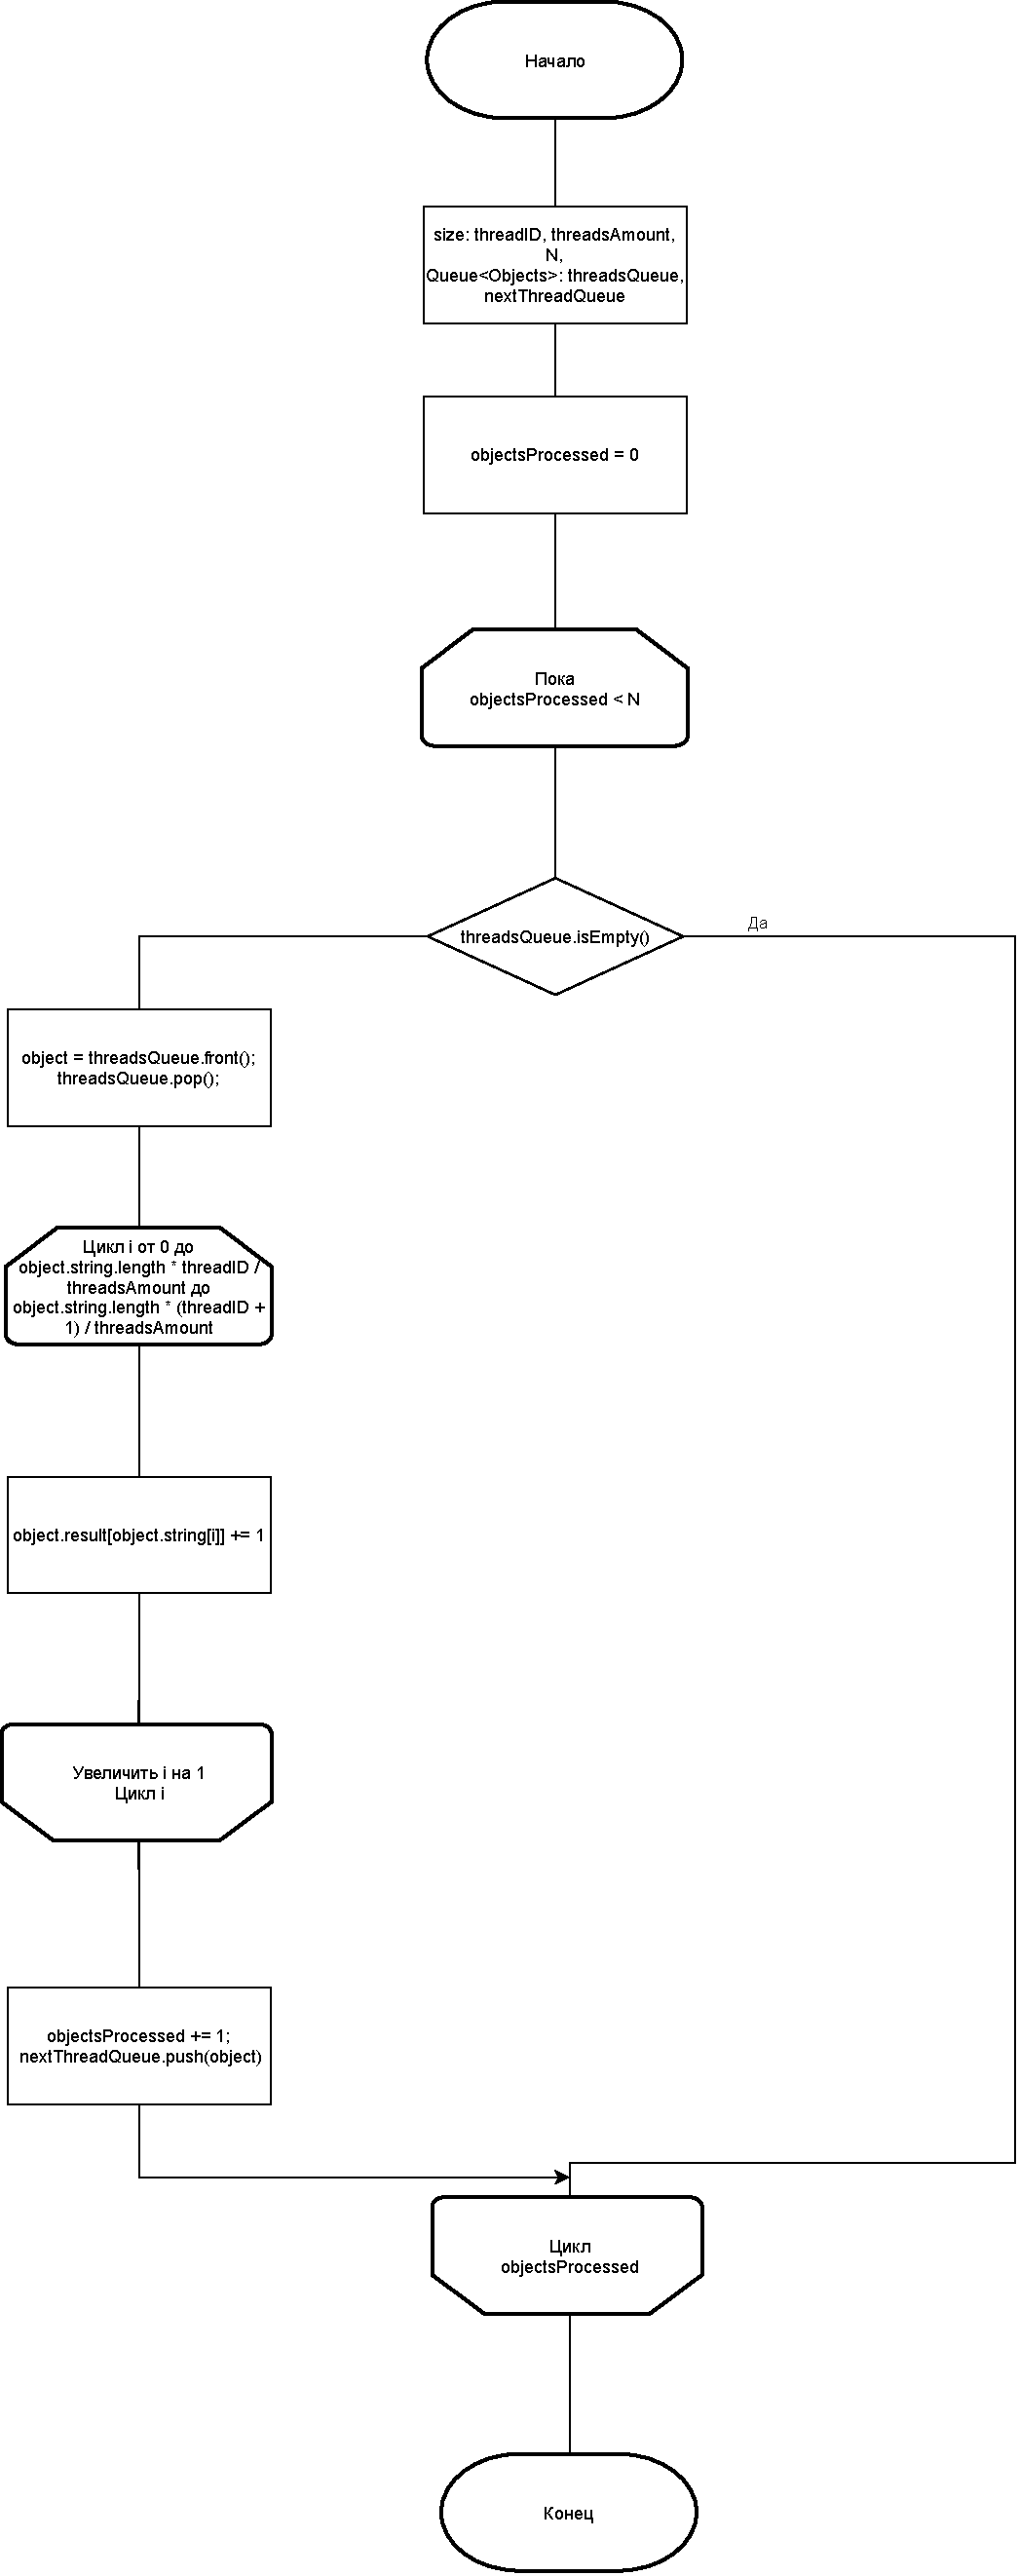
\includegraphics[width=.5\linewidth]{src/schemas/parallel_thread}\\
	Рис. 2.2.2: Cхема дочернего потока параллельного конвейерного алгоритма
\end{center}
\clearpage
\addcontentsline{toc}{subsection}{Вывод}
\section*{Вывод}
\qquad В данном разделе были рассмотрены схемы реализуемых алгоритмов.
\clearpage

\section{Технологическая часть}
\qquad В данном разделе будет описана технологическая часть лабораторной работы: требования к ПО, листинг кода, сравнительный анализ всех алгоритмов.
\subsection{Требования к программному обеспечению}
\qquad Входные данные: размерность массива строк, сами строки\\
\qquad Выходные данные: массивы, содержащие количество вхождений каждого из символов в каждой строке\\
\qquad Среда выполнения: Windows 10 x64
\qquad CPU:  Core i7-8550U
\subsection{Средства реализации}
\qquad Для выполнения данной лабораторной работы использовался язык программирования C++ стандарта 2020 года, а также среда разработки CLion 2020.2. Для замены времени было использовано средство \textbf{std::chrono} \cite{litlink4}
\subsection{Листинг кода}
\qquad В данном разделе будет представлен листинг кода разработанных алгоритмов.\\

Ниже, на листинге 3.1, представлена реализация последовательного алгоритма подсчёта:
\begin{center}
	Листинг 3.1: Последовательный алгоритм подсчёта
	\lstinputlisting[language=C++]{src/code/consistent.cpp}
\end{center}
\clearpage

Ниже, на листинге 3.2.1, представлена реализация главного потока параллельного конвейерного алгоритма подсчёта:
\begin{center}
	Листинг 3.2.1: Главный поток параллелльного конвейерного алгоритма подсчёта
	\lstinputlisting[language=C++]{src/code/parallel_main.cpp}
\end{center}

Ниже, на листинге 3.2.2, представлена реализация дочернего потока параллельного конвейерного алгоритма подсчёта:
\begin{center}
	Листинг 3.2.2: Дочерний поток параллельного конвейерного алгоритма подсчёта
	\lstinputlisting[language=C++]{src/code/parallel_thread.cpp}
\end{center}
\clearpage


\subsection{Описание тестирования} % описать, какие тесты будут проведены ВСЕ ТЕСТЫ ПРОЙДЕНЫ УСПЕШНО
Были проведены тесты на больших размерностях со случайными строками в качестве элементов.\\
Ниже, на листинге 3.3, представлен фрагмент кода тестирования корректной работы реализации алгоритмов
\begin{center}
	Листинг 3.3: Тестирование корректной работы алгоритмов
	\lstinputlisting[language=C++]{src/code/tests.cpp}	
\end{center}

Все тесты пройдены успешно.

\addcontentsline{toc}{subsection}{Вывод}
\section*{Вывод}
\qquad В данном разделе был представлен листинг реализованных алгоритмов, а также описание тестирование корректности их работы.
\clearpage

\section{Экспериментальная часть}
\qquad В данной части работы будут приведен анализ алгоритмов на основе эксперементальных данных.
\subsection{Сравнительный анализ на основе замеров времени работы алгоритмов}
Был проведён замер времени работы каждого из параллельных алгоритмов. Длина каждой строки 10000 символов. Каждый эксперимент на каждой размерности массива строк был произведён 5 раз, затем бралось среднее арифметическое полученного результата.\\
Для всех замеров количество конвейеров = 3.\\

Ниже, на графике 4.1, показана графическая интерпретация замеров времени работы\\

\begin{center}
	\begin{tikzpicture}
	\begin{axis}[
	axis lines = left,
	xlabel = {Количество строк},
	ylabel = {Время (с)},
	legend pos=north west,
	ymajorgrids=true
	]
	\addplot[color=red, mark=square] table[x index=0, y index= 1] {src/graph/consistent.txt};
	\addlegendentry{Последовательный конвейер}
	
	\addplot[color=blue, mark=square] table[x index=0, y index= 1] {src/graph/parallel.txt};
	\addlegendentry{Параллельный конвейер}
	\end{axis}
	\end{tikzpicture}\\
	График 4.1: Замеры вермени работы первого параллельного алгоритма\\
\end{center}

\section*{Вывод}
По результатам исследования выяснилось, что при малых размерностях входных данных разница по времени между алгоритмами не существенна, но с увелечением размерности разница становится всё больше и больше.
\clearpage

\addcontentsline{toc}{section}{Заключение}
\section*{\Huge Заключение}
\qquad В ходе работы были изучен алгоритм нахождения количества вхождений каждого символа в наборе строк, а также разработаны 2 конвейреные версии этого алгоритма: последовательный и параллельный. Экспериментально было установлено, что параллельная версии быстрее последовательной алгоритма.
%//////////////////////////////////////////////////////////////////
\clearpage
\renewcommand\refname{Список использованной литературы}
\addcontentsline{toc}{section}{Список использованной литературы}
\begin{thebibliography}{}
	\bibitem{litlink1} Справка по потокам в ОС Windows // https://docs.microsoft.com/en-us/windows/win32/procthread/process-and-thread-functions (дата обращения: 27.10.2020).
	\bibitem{litlink2} Кнут Д. Э. Искусство программирования. Том 1. Сортировка и поиск . -- М.: Вильямс, 2007. -- 832 с.
	\bibitem{litlink3} Богачев К.Ю Основы параллельного программирования. -- М.: БИНОМ. Лаборатория знаний 2003.  -- 237 с.
	\bibitem{litlink4} Справка по C++ // cppreference URL: https://en.cppreference.com/w/ (дата обращения: 27.10.2020).
\end{thebibliography}
\end{document}